% Options for packages loaded elsewhere
\PassOptionsToPackage{unicode}{hyperref}
\PassOptionsToPackage{hyphens}{url}
%
\documentclass[
]{book}
\usepackage{amsmath,amssymb}
\usepackage{lmodern}
\usepackage{ifxetex,ifluatex}
\ifnum 0\ifxetex 1\fi\ifluatex 1\fi=0 % if pdftex
  \usepackage[T1]{fontenc}
  \usepackage[utf8]{inputenc}
  \usepackage{textcomp} % provide euro and other symbols
\else % if luatex or xetex
  \usepackage{unicode-math}
  \defaultfontfeatures{Scale=MatchLowercase}
  \defaultfontfeatures[\rmfamily]{Ligatures=TeX,Scale=1}
\fi
% Use upquote if available, for straight quotes in verbatim environments
\IfFileExists{upquote.sty}{\usepackage{upquote}}{}
\IfFileExists{microtype.sty}{% use microtype if available
  \usepackage[]{microtype}
  \UseMicrotypeSet[protrusion]{basicmath} % disable protrusion for tt fonts
}{}
\makeatletter
\@ifundefined{KOMAClassName}{% if non-KOMA class
  \IfFileExists{parskip.sty}{%
    \usepackage{parskip}
  }{% else
    \setlength{\parindent}{0pt}
    \setlength{\parskip}{6pt plus 2pt minus 1pt}}
}{% if KOMA class
  \KOMAoptions{parskip=half}}
\makeatother
\usepackage{xcolor}
\IfFileExists{xurl.sty}{\usepackage{xurl}}{} % add URL line breaks if available
\IfFileExists{bookmark.sty}{\usepackage{bookmark}}{\usepackage{hyperref}}
\hypersetup{
  pdftitle={Proyecto Final: Hotel Cancelation},
  pdfauthor={Alex Joel Marco},
  hidelinks,
  pdfcreator={LaTeX via pandoc}}
\urlstyle{same} % disable monospaced font for URLs
\usepackage{color}
\usepackage{fancyvrb}
\newcommand{\VerbBar}{|}
\newcommand{\VERB}{\Verb[commandchars=\\\{\}]}
\DefineVerbatimEnvironment{Highlighting}{Verbatim}{commandchars=\\\{\}}
% Add ',fontsize=\small' for more characters per line
\usepackage{framed}
\definecolor{shadecolor}{RGB}{248,248,248}
\newenvironment{Shaded}{\begin{snugshade}}{\end{snugshade}}
\newcommand{\AlertTok}[1]{\textcolor[rgb]{0.94,0.16,0.16}{#1}}
\newcommand{\AnnotationTok}[1]{\textcolor[rgb]{0.56,0.35,0.01}{\textbf{\textit{#1}}}}
\newcommand{\AttributeTok}[1]{\textcolor[rgb]{0.77,0.63,0.00}{#1}}
\newcommand{\BaseNTok}[1]{\textcolor[rgb]{0.00,0.00,0.81}{#1}}
\newcommand{\BuiltInTok}[1]{#1}
\newcommand{\CharTok}[1]{\textcolor[rgb]{0.31,0.60,0.02}{#1}}
\newcommand{\CommentTok}[1]{\textcolor[rgb]{0.56,0.35,0.01}{\textit{#1}}}
\newcommand{\CommentVarTok}[1]{\textcolor[rgb]{0.56,0.35,0.01}{\textbf{\textit{#1}}}}
\newcommand{\ConstantTok}[1]{\textcolor[rgb]{0.00,0.00,0.00}{#1}}
\newcommand{\ControlFlowTok}[1]{\textcolor[rgb]{0.13,0.29,0.53}{\textbf{#1}}}
\newcommand{\DataTypeTok}[1]{\textcolor[rgb]{0.13,0.29,0.53}{#1}}
\newcommand{\DecValTok}[1]{\textcolor[rgb]{0.00,0.00,0.81}{#1}}
\newcommand{\DocumentationTok}[1]{\textcolor[rgb]{0.56,0.35,0.01}{\textbf{\textit{#1}}}}
\newcommand{\ErrorTok}[1]{\textcolor[rgb]{0.64,0.00,0.00}{\textbf{#1}}}
\newcommand{\ExtensionTok}[1]{#1}
\newcommand{\FloatTok}[1]{\textcolor[rgb]{0.00,0.00,0.81}{#1}}
\newcommand{\FunctionTok}[1]{\textcolor[rgb]{0.00,0.00,0.00}{#1}}
\newcommand{\ImportTok}[1]{#1}
\newcommand{\InformationTok}[1]{\textcolor[rgb]{0.56,0.35,0.01}{\textbf{\textit{#1}}}}
\newcommand{\KeywordTok}[1]{\textcolor[rgb]{0.13,0.29,0.53}{\textbf{#1}}}
\newcommand{\NormalTok}[1]{#1}
\newcommand{\OperatorTok}[1]{\textcolor[rgb]{0.81,0.36,0.00}{\textbf{#1}}}
\newcommand{\OtherTok}[1]{\textcolor[rgb]{0.56,0.35,0.01}{#1}}
\newcommand{\PreprocessorTok}[1]{\textcolor[rgb]{0.56,0.35,0.01}{\textit{#1}}}
\newcommand{\RegionMarkerTok}[1]{#1}
\newcommand{\SpecialCharTok}[1]{\textcolor[rgb]{0.00,0.00,0.00}{#1}}
\newcommand{\SpecialStringTok}[1]{\textcolor[rgb]{0.31,0.60,0.02}{#1}}
\newcommand{\StringTok}[1]{\textcolor[rgb]{0.31,0.60,0.02}{#1}}
\newcommand{\VariableTok}[1]{\textcolor[rgb]{0.00,0.00,0.00}{#1}}
\newcommand{\VerbatimStringTok}[1]{\textcolor[rgb]{0.31,0.60,0.02}{#1}}
\newcommand{\WarningTok}[1]{\textcolor[rgb]{0.56,0.35,0.01}{\textbf{\textit{#1}}}}
\usepackage{longtable,booktabs,array}
\usepackage{calc} % for calculating minipage widths
% Correct order of tables after \paragraph or \subparagraph
\usepackage{etoolbox}
\makeatletter
\patchcmd\longtable{\par}{\if@noskipsec\mbox{}\fi\par}{}{}
\makeatother
% Allow footnotes in longtable head/foot
\IfFileExists{footnotehyper.sty}{\usepackage{footnotehyper}}{\usepackage{footnote}}
\makesavenoteenv{longtable}
\usepackage{graphicx}
\makeatletter
\def\maxwidth{\ifdim\Gin@nat@width>\linewidth\linewidth\else\Gin@nat@width\fi}
\def\maxheight{\ifdim\Gin@nat@height>\textheight\textheight\else\Gin@nat@height\fi}
\makeatother
% Scale images if necessary, so that they will not overflow the page
% margins by default, and it is still possible to overwrite the defaults
% using explicit options in \includegraphics[width, height, ...]{}
\setkeys{Gin}{width=\maxwidth,height=\maxheight,keepaspectratio}
% Set default figure placement to htbp
\makeatletter
\def\fps@figure{htbp}
\makeatother
\setlength{\emergencystretch}{3em} % prevent overfull lines
\providecommand{\tightlist}{%
  \setlength{\itemsep}{0pt}\setlength{\parskip}{0pt}}
\setcounter{secnumdepth}{5}
\usepackage{booktabs}
\ifluatex
  \usepackage{selnolig}  % disable illegal ligatures
\fi
\usepackage[]{natbib}
\bibliographystyle{apalike}

\title{Proyecto Final: Hotel Cancelation}
\author{Alex Joel Marco}
\date{2021-12-05}

\begin{document}
\maketitle

{
\setcounter{tocdepth}{1}
\tableofcontents
}
\hypertarget{introducciuxf3n}{%
\chapter{Introducción}\label{introducciuxf3n}}

\hypertarget{proyecto}{%
\section{Proyecto}\label{proyecto}}

\begin{itemize}
\tightlist
\item
  Cancelaciones en Hoteles
\item
  Predecir cancelación de reservas en hoteles - AM 2021
\end{itemize}

\hypertarget{descripciuxf3n-del-problema}{%
\section{Descripción del problema}\label{descripciuxf3n-del-problema}}

Con el fin de planear tarifas y actividades de ventas o promoción, los hoteles hacen estimaciones adelantadas de su ocupación en cada día. Una parte de estas estimaciones requiere predecir cuántas de las reservaciones que ya se tienen van a terminar en cancelaciones, lo cual libera inventario que afecta en la planeación.

\hypertarget{objetivo}{%
\section{Objetivo}\label{objetivo}}

Predecir cuáles reservaciones son probables que terminen o no en cancelación.

\hypertarget{fuente-de-datos}{%
\section{Fuente de datos}\label{fuente-de-datos}}

Los datos que se utilizaron para este proyecto fueron obtenidos del sitio

\url{https://www.kaggle.com/c/cancelaciones-en-hoteles/data}

Los datos originales provienen de Hotel booking demand datasets, Antonio, de Almeida, Nunes (\url{https://www.sciencedirect.com/science/article/pii/S2352340918315191})

\hypertarget{ambiente}{%
\section{Ambiente}\label{ambiente}}

\hypertarget{analisis-exploratorio-de-datos}{%
\chapter{Analisis Exploratorio de Datos}\label{analisis-exploratorio-de-datos}}

Con el fin de entender los datos realizamos una revisión general de estos (solamente de la base de datos de entrenamiento posterior a haberla dividido en entrenamiento, validación y prueba) y tratamos de identificar aquellas variables que pudieran ser interesantes para nuestro estudio. A continuación se muestra una breve parte de la exploración de datos. Si desea consultar el análisis completo puede encontrarlo en la siguiente liga \href{https://github.com/marcoyel21/hotel_cancelation_ML21/blob/main/final/EDA_Cancelaciones.Rmd}{EDA}.

El data set está compuesto por las siguientes variables:

\begin{longtable}[]{@{}
  >{\centering\arraybackslash}p{(\columnwidth - 4\tabcolsep) * \real{0.33}}
  >{\centering\arraybackslash}p{(\columnwidth - 4\tabcolsep) * \real{0.33}}
  >{\centering\arraybackslash}p{(\columnwidth - 4\tabcolsep) * \real{0.33}}@{}}
\toprule
Variable & Tipo & Descripción \\ \addlinespace
\midrule
\endhead
ADR & Numeric & Tarifa diaria promedio definida por {[}5{]} \\ \addlinespace
Adults & Integer & Número de Adultos \\ \addlinespace
Agent & Categorical & DNI de la agencia de viajes que realizó la reservaa \\ \addlinespace
ArrivalDateDayOfMonth & Integer & Día del mes de la fecha de llegada \\ \addlinespace
ArrivalDateMonth & Categorical & Mes de la fecha de llegada con 12 categorías: ``enero'' a ``diciembre'' \\ \addlinespace
ArrivalDateWeekNumber & Integer & Número de semana de la fecha de llegada \\ \addlinespace
ArrivalDateYear & Integer & Año de la fecha de llegada \\ \addlinespace
AssignedRoomType & Categorical & Código del tipo de habitación asignada a la reserva. A veces, el tipo de habitación asignada difiere del tipo de habitación reservada debido a razones de operación del hotel (por ejemplo, overbooking) o por solicitud del cliente. El código se presenta en lugar de la designación por razones de anonimato \\ \addlinespace
Babies & Integer & Numero de bebes \\ \addlinespace
BookingChanges & Integer & Número de cambios / modificaciones realizadas a la reserva desde el momento en que se ingresó la reserva en el PMS hasta el momento del check-in o la cancelación \\ \addlinespace
Children & Integer & Numero de niños \\ \addlinespace
Company & Categorical & DNI de la empresa / entidad que realizó la reserva o responsable del pago de la reserva. La identificación se presenta en lugar de la designación por razones de anonimato \\ \addlinespace
Country & Categorical & País de origen. Las categorías están representadas en el formato ISO 3155-3: 2013 {[}6{]} \\ \addlinespace
CustomerType & Categorical & Tipo de reserva, asumiendo una de cuatro categorías: \\ \addlinespace
DaysInWaitingList & Integer & Número de días que la reserva estuvo en lista de espera antes de que fuera confirmada al cliente \\ \addlinespace
DepositType & Categorical & Indicación sobre si el cliente realizó un depósito para garantizar la reserva. Esta variable puede asumir tres categorías: \\ \addlinespace
DistributionChannel & Categorical & Canal de distribución de reservas. El término ``TA'' significa ``Agentes de viajes'' y ``TO'' significa ``Operadores turísticos'' \\ \addlinespace
\textbf{IsCanceled} & \textbf{Categorical} & \textbf{Valor que indica si la reserva fue cancelada (1) o no (0)} \\ \addlinespace
IsRepeatedGuest & Categorical & Valor que indica si el nombre de la reserva fue de un huésped repetido (1) o no (0) \\ \addlinespace
LeadTime & Integer & Número de días transcurridos entre la fecha de entrada de la reserva en el PMS y la fecha de llegada \\ \addlinespace
MarketSegment & Categorical & Designación de segmento de mercado. En las categorías, el término ``TA'' significa ``Agentes de viajes'' y ``TO'' significa ``Operadores turísticos'' \\ \addlinespace
Meal & Categorical & Tipo de comida reservada. Las categorías se presentan en paquetes de comidas de hospitalidad estándar: \\ \addlinespace
PreviousBookingsNotCanceled & Integer & Número de reservas anteriores no canceladas por el cliente antes de la reserva actual \\ \addlinespace
PreviousCancellations & Integer & Número de reservas anteriores que fueron canceladas por el cliente antes de la reserva actual \\ \addlinespace
RequiredCardParkingSpaces & Integer & Número de plazas de aparcamiento requeridas por el cliente \\ \addlinespace
ReservationStatus & Categorical & Último estado de la reserva, asumiendo una de tres categorías: \\ \addlinespace
ReservationStatusDate & Date & Fecha en la que se estableció el último estado. Esta variable se puede utilizar junto con ReservationStatus para comprender cuándo se canceló la reserva o cuándo se registró el cliente en el hotel. \\ \addlinespace
ReservedRoomType & Categorical & Código del tipo de habitación reservado. El código se presenta en lugar de la designación por razones de anonimato \\ \addlinespace
StaysInWeekendNights & Integer & Número de noches de fin de semana (sábado o domingo) que el huésped se hospedó o reservó para alojarse en el hotel \\ \addlinespace
StaysInWeekNights & Integer & Número de noches de la semana (de lunes a viernes) que el huésped se hospedó o reservó para alojarse en el hotel \\ \addlinespace
TotalOfSpecialRequests & Integer & Número de solicitudes especiales realizadas por el cliente (por ejemplo, dos camas individuales o piso alto) \\ \addlinespace
\bottomrule
\end{longtable}

Nuestra variable de interés es \textbf{IsCanceled} la cual toma valores de 1 (fue cancelada) y 0 (no fue cancelada). Así que primero veamos la proporción de cancelaciones en los datos.

\begin{longtable}[]{@{}cc@{}}
\toprule
Cancelado & No cancelado \\ \addlinespace
\midrule
\endhead
0.3620854 & 0.6379146 \\ \addlinespace
\bottomrule
\end{longtable}

Usamos la función skim en la base de datos de entrenamiento para conocer las características generales de cada variable.

Podemos observar que:

\begin{itemize}
\item
  Tenemos 13 variables categorías, de las cuales podemos destacar que 3 tienen un número alto de categorías (country, agent, company).
\item
  Tenemos 17 variables numéricas.
\item
  En este primer acercamiento, podemos identificar que las variables corresponden a:

  \begin{itemize}
  \item
    Variables de tiempo: tiempo previo de reservación, fechas de llegada, duración de la reservación.
  \item
    Características de reservación: agencia, país, canal de distribución, segmento de mercado, tipo de depósito, tarifa diaria
  \item
    Características de los clientes y sus preferencias: adultos, bebes, tipo de hotel, tipo de habitación
  \end{itemize}
\end{itemize}

\hypertarget{cancelaciones-eda}{%
\subsection{Cancelaciones EDA}\label{cancelaciones-eda}}

Ahora extraemos el subconjunto de cancelados para hacer una revisión de todas las variables con respecto a las reservaciónes canceladas.

\begin{Shaded}
\begin{Highlighting}[]
\NormalTok{sub\_cancelados }\OtherTok{\textless{}{-}} \FunctionTok{subset}\NormalTok{(train, is\_canceled }\SpecialCharTok{==} \StringTok{"cancelado"}\NormalTok{)}
\end{Highlighting}
\end{Shaded}

Iniciamos con la revisión de los histogramas de cada variable para ver si podemos identificar algun compartamiento interesante. A continuación se muestran los histogramas de las variables más interesantes a nuestro criterio, nuevamente puede consultar la exploración completa de los datos en \href{https://github.com/marcoyel21/hotel_cancelation_ML21/blob/main/final/EDA_Cancelaciones.Rmd}{EDA}.

\textbf{Lead\_time:} la distribución de sus datos no tiene un comportamiento lógico, porque el mayor número de cancelaciones proviene de o días previos de reservación, pero luego se mueve a valores de 90 días, 40 días y luego regresa a 2 días. será importante ver si existe algún patrón en esta variable.

\begin{center}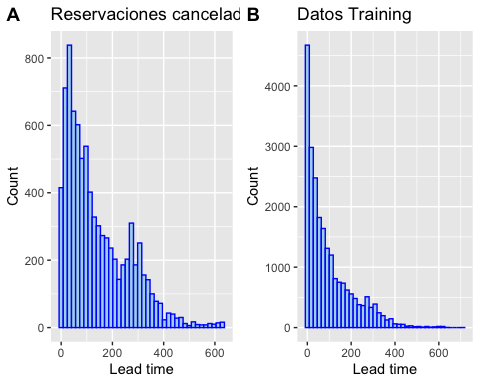
\includegraphics{final_bookdown_files/figure-latex/unnamed-chunk-4-1} \end{center}

\textbf{Agregar comparacion poblaciones} \#\#\#\#\#\#\#\#\#\#\#\#\#\#\#\#\#\#\#\#\#\#\#\#\#\#\#\#\#\#\#\#\#\#\#\#\#\#\#\#\#\#
\#\#\#\#\#\#\#\#\#\#\#\#\#\#\#\#\#\#\#\#\#\#\#\#\#\#\#\#\#\#\#\#\#\#\#\#\#\#\#\#\#\#\#\#\#\#\#\#\#

\textbf{Country:} esta variable presenta un dato totalmente atípico en la categoría PRT por lo que es importante considerarla ya que podría explicar una porción importante de las cancelaciones.

\begin{Shaded}
\begin{Highlighting}[]
\CommentTok{\#![ ](country.png) }
\end{Highlighting}
\end{Shaded}

\textbf{Deposit\_type:} aqui hay otro caso ilógico, ya que la categoría de no rembolsable está muy por arriba de los rembolsable, uno pensaría que debería ser menos frecuenta la cancelación si no te van a devolver tu dinero. por lo que es otra variable importante.

\begin{center}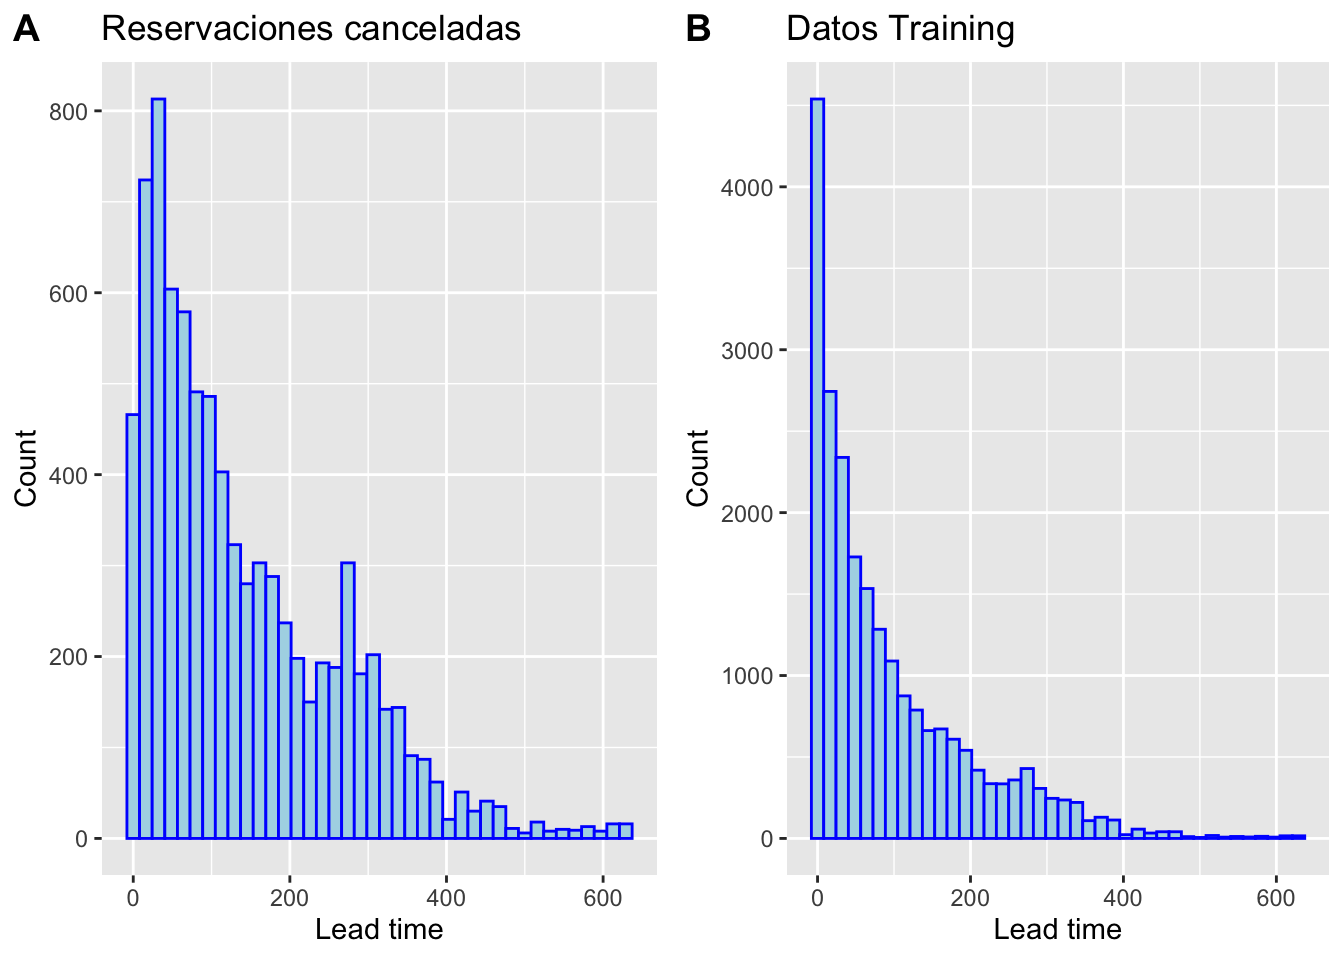
\includegraphics{final_bookdown_files/figure-latex/unnamed-chunk-6-1} \end{center}

Analisando la variable \textbf{deposit\_type}, se extrae el subset de deposit\_type cancelados. Revisamos los porcentajes de cada categoría en las otras variables y observamos que el 97\% de las cancelaciones sin rembolso pertenecen al país PRT.

\begin{verbatim}
## 
##          BEL           CN          ESP          FRA          GBR         NULL 
## 0.0016966407 0.0016966407 0.0108585002 0.0010179844 0.0122158127 0.0003393281 
##          POL          PRT 
## 0.0037326094 0.9684424839
\end{verbatim}

\textbf{Joel} añadir descubrimientos agent 1 portugal discucsión

\hypertarget{anuxe1lisis-de-tendenciuxe1s-en-el-tiempo-eda}{%
\subsection{Análisis de tendenciás en el tiempo EDA}\label{anuxe1lisis-de-tendenciuxe1s-en-el-tiempo-eda}}

Para analizar tendencias de cancelación en el timepo se agrupan las cancelaciones por fecha.

\begin{center}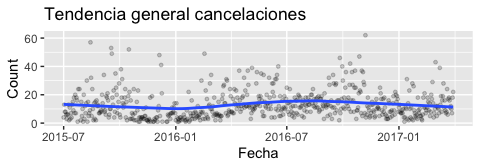
\includegraphics[width=0.9\linewidth]{final_bookdown_files/figure-latex/unnamed-chunk-9-1} \end{center}

Se procede a hacer un análisis de \href{https://es.wikipedia.org/wiki/Serie_temporal}{series de tiempo}.

\begin{center}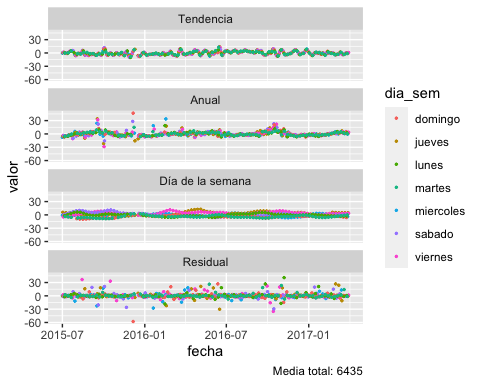
\includegraphics{final_bookdown_files/figure-latex/unnamed-chunk-11-1} \end{center}

\textbf{Joel} Analisis días de la semana

\begin{center}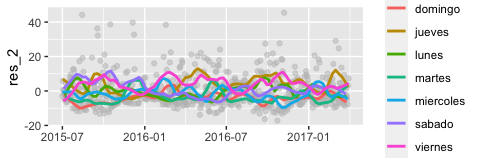
\includegraphics[width=0.9\linewidth]{final_bookdown_files/figure-latex/unnamed-chunk-12-1} \end{center}

\textbf{Joel} Picos durante el año

\begin{center}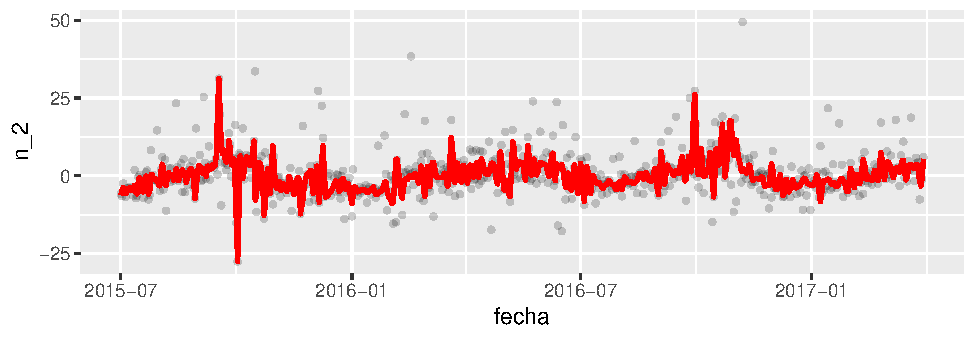
\includegraphics[width=0.9\linewidth]{final_bookdown_files/figure-latex/unnamed-chunk-13-1} \end{center}

\hypertarget{preparaciuxf3n-de-los-datos}{%
\chapter{Preparación de los Datos}\label{preparaciuxf3n-de-los-datos}}

\hypertarget{preprocesamiento}{%
\subsection{Preprocesamiento}\label{preprocesamiento}}

\begin{itemize}
\item
  Muchos datos necesitan preprocesamiento sobretodo porque están codificados como ``character'' en lugar de ``factor'': por ejemplo, las variables: arrival\_date\_year,arrival\_date\_month,arrival\_date\_week\_number,meal,country,market\_segment,distribution\_channel,agent,company,customer\_type, hotel,agent\_company.reserved\_room\_type,assigned\_room\_type,deposit\_type.
\item
  Otros necesitan ser números: children
\end{itemize}

\hypertarget{ingenieruxeda-de-caracteruxedsitcas}{%
\subsection{Ingeniería de caracterísitcas}\label{ingenieruxeda-de-caracteruxedsitcas}}

Para el preprocesamiento de datos se agregaron variables que pensamos serían de utilidad. Entre estas nuevas variables se encuentran:

\begin{itemize}
\item
  \textbf{lead\_time}: Se cuentan los días de anticipación de la reserva y se divide en 4 grandes grupos del mismo tamaño.
\item
  \textbf{dif\_room}: Esta variable toma en cuenta si la habitación reservada es la misma que la habitación asignada.
\item
  \textbf{singles\_adults}: Indica si hay solo adultos (sin niños)
\item
  \textbf{pascua, pascua\_m1, \ldots., pascua\_m6 }: indica si tal fecha era Pascua.
\item
  \textbf{mag\_tasa\_can}: Proporciona el ratio entre el total de cancelaciones respecto al total de reservaciones.
\end{itemize}

** \textbf{COMBINACIONES aleatorias}: Incorporamos estas variables de combinaciones al azar buscando interaciones que ayudaran al modelo.*
\#\#\# Combinaciónes

Asimismo exploramos distintas combinaciones pensando en que los modelos que ibamos a usar tenían la capacidad de seleccionar automáticamente las caracterísitcas más útiles.

\begin{itemize}
\item
  \textbf{dias\_semana}: Interaccion entre el día de reservación y el número de semana.
\item
  \textbf{Agent\_company}: La combinación de agent y company.Esta resulto muy util en los casos donde ambas variables tenían valor NULL.
\item
  \textbf{dif\_room}: Si el cuarto asignado es diferente al cuarto reservado.
\item
  \textbf{week\_day\_sem}: Combinación de día de la semana y número de semana.
\item
  \textbf{week\_daymonth}: Combinación de día de la semana y número de semana.
\item
  \textbf{Tasa de rechazo}: Proporcion de reservaciones canceladas del total de reservaciones registradas.
\item
  \textbf{market\_dist}: Combinación de market\_segment y distribution\_chanel.
\item
  \textbf{cust\_deposti}:Combinación de customer\_type y deposit\_type.
\item
  \textbf{cust\_segment}: Combinación de customer\_type y market\_segment.
\item
  \textbf{lead\_deposit}: Combinación de lead y del tipo de deposito.
\item
  \textbf{lead\_week}: Combinación de lead y número de semana de la reserva.
\item
  \textbf{meal\_reserv}: Combinación de tipo de alimento y tipo de reserva.
\item
  \textbf{country\_month}: Combinación del mes de la reserva y el país de origen.
\end{itemize}

\hypertarget{cv}{%
\section{CV}\label{cv}}

Ahora sobre el conjunto de entrenamiento guardaremos un cacho para probar.

\begin{Shaded}
\begin{Highlighting}[]
\CommentTok{\# proporción que queremos de training}
\NormalTok{training\_size }\OtherTok{\textless{}{-}} \FloatTok{0.8}
\CommentTok{\# filas de training}
\NormalTok{training\_rows }\OtherTok{\textless{}{-}} \FunctionTok{sample}\NormalTok{(}\FunctionTok{seq\_len}\NormalTok{(}\FunctionTok{nrow}\NormalTok{(newdata\_train)),}
                        \AttributeTok{size=}\FunctionTok{floor}\NormalTok{(training\_size}\SpecialCharTok{*}\FunctionTok{nrow}\NormalTok{(newdata\_train)))}
\CommentTok{\#training set}
\NormalTok{data\_training }\OtherTok{\textless{}{-}}\NormalTok{ newdata\_train[training\_rows,]}
\CommentTok{\#training cuenta con la y}


\CommentTok{\#validation set}
\CommentTok{\# la variable objetivo por separado}
\NormalTok{data\_validation }\OtherTok{\textless{}{-}}\NormalTok{ newdata\_train[}\SpecialCharTok{{-}}\NormalTok{training\_rows,}\SpecialCharTok{{-}}\DecValTok{1}\NormalTok{] }\CommentTok{\#sin la y}
\NormalTok{y }\OtherTok{\textless{}{-}}\NormalTok{ newdata\_train[}\SpecialCharTok{{-}}\NormalTok{training\_rows,}\DecValTok{1}\NormalTok{] }
\end{Highlighting}
\end{Shaded}

\hypertarget{nivelaciuxf3n-de-variables}{%
\section{Nivelación de variables}\label{nivelaciuxf3n-de-variables}}

Antes de realizar la conversión a matrices ralas necesitamos indicarle a la computadora que las bases de datos cuentan con los mismas variables y dentro de cada variable categórica, los mismos niveles. Esto debido a que al hacer el CV, es muy probable que no todas las variables conserven la misma cantidad de niveles que la base completa antes del CV. Para ello creamos la siguiente función y la aplicamos a las bases de datos.

\begin{Shaded}
\begin{Highlighting}[]
\CommentTok{\# creo una funcion para que las bases de datos cuenten con los mismos "levels"}
\CommentTok{\# este paso es crucial para asegurarnos que traning, set y el modelo hablen "el mismo idioma", es decir que tengan las mismas variables}
\NormalTok{equallevels }\OtherTok{\textless{}{-}} \ControlFlowTok{function}\NormalTok{(x, y) \{}
    \ControlFlowTok{if}\NormalTok{ (}\FunctionTok{is.data.frame}\NormalTok{(x) }\SpecialCharTok{\&} \FunctionTok{is.data.frame}\NormalTok{(y)) \{}
\NormalTok{        com }\OtherTok{\textless{}{-}} \FunctionTok{intersect}\NormalTok{(}\AttributeTok{x =} \FunctionTok{names}\NormalTok{(x), }\AttributeTok{y =} \FunctionTok{names}\NormalTok{(y))}
        \ControlFlowTok{for}\NormalTok{ (i }\ControlFlowTok{in}\NormalTok{ com) \{}
            \ControlFlowTok{if}\NormalTok{ (}\SpecialCharTok{!}\FunctionTok{is.null}\NormalTok{(}\FunctionTok{levels}\NormalTok{(y[[i]]))) \{}
\NormalTok{                x[[i]] }\OtherTok{\textless{}{-}} \FunctionTok{factor}\NormalTok{(x[[i]], }\AttributeTok{levels =} \FunctionTok{levels}\NormalTok{(y[[i]]))}
\NormalTok{            \}}
\NormalTok{        \}}
        \FunctionTok{return}\NormalTok{(x)}
\NormalTok{    \} }\ControlFlowTok{else}\NormalTok{ \{}
        \FunctionTok{stop}\NormalTok{(}\StringTok{"\textasciigrave{}x\textasciigrave{} and \textasciigrave{}y\textasciigrave{} must be a data.frame."}\NormalTok{)}
\NormalTok{    \}}
\NormalTok{\}}
\end{Highlighting}
\end{Shaded}

\hypertarget{matrices-ralas}{%
\section{Matrices RALAS}\label{matrices-ralas}}

Para el procesamiento de los datos previo al modelaje se hizo \href{https://www.educative.io/blog/one-hot-encoding}{one hot encoding}, el cuál consiste en transformar las variables categóricas en variables dummy. Cómo ya se mencionó en el EDA, existen variables con muchísimas categorías (country, agent, company). Lo cual nos deja con un data frame lleno de muchos ceros. Para manejar este ``data frame'' o ``matriz'' con muchos ceros se hizo uso de las \href{http://amunategui.github.io/sparse-matrix-glmnet/}{matrices Ralas} las cuales concervan únicamente las entradas con valores distintos de cero. Para ello se utilizó la función \textbf{sparse.model.matrix} de la librería \href{https://cran.rproject.org/web/packages/Matrix/index.html}{Matrix}. La implementación del código completa la puede ver en la siguiente liga \href{https://github.com/marcoyel21/hotel_cancelation_ML21/blob/main/final/modelo_final\%20.Rmd}{Model}.

\begin{Shaded}
\begin{Highlighting}[]
\CommentTok{\#![Ejemplo trasfomación matriz a matriz ralas ](ralas.png)}
\end{Highlighting}
\end{Shaded}

\begin{Shaded}
\begin{Highlighting}[]
\CommentTok{\#Matriz de covariates}
\CommentTok{\#data\_training\textless{}{-}sample\_train}
\NormalTok{Xa }\OtherTok{\textless{}{-}}\NormalTok{data\_training }\SpecialCharTok{\%\textgreater{}\%} \FunctionTok{select}\NormalTok{(}\SpecialCharTok{{-}}\DecValTok{1}\NormalTok{) }\CommentTok{\#training menos y}
\NormalTok{Xb }\OtherTok{\textless{}{-}}\NormalTok{data\_validation}
\NormalTok{Xc }\OtherTok{\textless{}{-}}\FunctionTok{equallevels}\NormalTok{(newdata\_test,Xa)}

\CommentTok{\#para manejo de nas, si lo quito, por alguna razon la conversion a matriz rala me quita unas obs}

\FunctionTok{options}\NormalTok{(}\AttributeTok{na.action=}\StringTok{\textquotesingle{}na.pass\textquotesingle{}}\NormalTok{)}
\end{Highlighting}
\end{Shaded}

Ahora creo 3 matrices ralas para entrenamiento, validación y prueba.

\begin{Shaded}
\begin{Highlighting}[]
\CommentTok{\#se quita intercepto}
\CommentTok{\#se ponen todas las columnas}
\NormalTok{Xa }\OtherTok{\textless{}{-}} \FunctionTok{sparse.model.matrix}\NormalTok{(}\SpecialCharTok{\textasciitilde{}}\NormalTok{.}\SpecialCharTok{+}\DecValTok{0}\NormalTok{, }\AttributeTok{data =}\NormalTok{ Xa)}
\NormalTok{Xb }\OtherTok{\textless{}{-}} \FunctionTok{sparse.model.matrix}\NormalTok{(}\SpecialCharTok{\textasciitilde{}}\NormalTok{.}\SpecialCharTok{+}\DecValTok{0}\NormalTok{, }\AttributeTok{data =}\NormalTok{ Xb)}
\NormalTok{Xc }\OtherTok{\textless{}{-}} \FunctionTok{sparse.model.matrix}\NormalTok{(}\SpecialCharTok{\textasciitilde{}}\NormalTok{.}\SpecialCharTok{+}\DecValTok{0}\NormalTok{, }\AttributeTok{data =}\NormalTok{ Xc)}

\CommentTok{\#vector de Y´s}
\NormalTok{Ya}\OtherTok{\textless{}{-}}\NormalTok{data\_training}\SpecialCharTok{$}\NormalTok{y}
\end{Highlighting}
\end{Shaded}

Ahora tengo 3 matrices con una alta cantidad de variables(4,347) (debido al one hot encoding y a la nivelación) para cada dataset del CV. Esto pensando en el feature seleccion que los modelos pueden hacer. Ahora puedo aplicarles cualquier modelo de manera muy ordenada y simple.

\hypertarget{modeling}{%
\chapter{Modeling}\label{modeling}}

En esta parte aplicaremos dos modelos: un Lasso-Logit y un XGboosting.

\hypertarget{cross-validated-lasso-logit}{%
\section{Cross-Validated LASSO-logit}\label{cross-validated-lasso-logit}}

Seestima un cross validated LASSO y se muestra el la gráfica de CV Binomial Deviance vs Complejidad

\begin{Shaded}
\begin{Highlighting}[]
\CommentTok{\#CV LASSO}
\CommentTok{\# se hacen 5 folds }
\NormalTok{cvlasso\_a}\OtherTok{\textless{}{-}}\FunctionTok{cv.gamlr}\NormalTok{(}\AttributeTok{x =}\NormalTok{ Xa, }\AttributeTok{y =}\NormalTok{ Ya, }\AttributeTok{verb =}\NormalTok{ T, }\AttributeTok{family =} \StringTok{\textquotesingle{}binomial\textquotesingle{}}\NormalTok{, }\AttributeTok{nfold =} \DecValTok{5}\NormalTok{)}
\end{Highlighting}
\end{Shaded}

\begin{verbatim}
## Warning in gamlr(x, y, ...): numerically perfect fit for some observations.
\end{verbatim}

\begin{verbatim}
## fold 1,2,3,4,5,done.
\end{verbatim}

\begin{Shaded}
\begin{Highlighting}[]
\CommentTok{\#Grafica}
\FunctionTok{plot}\NormalTok{(cvlasso\_a)}
\end{Highlighting}
\end{Shaded}

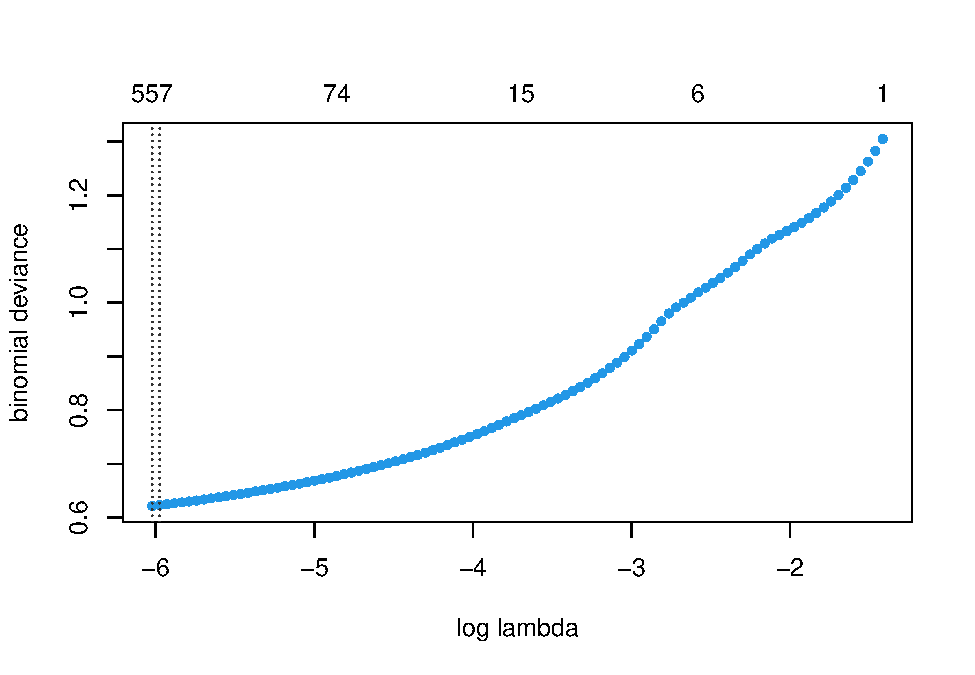
\includegraphics{final_bookdown_files/figure-latex/unnamed-chunk-22-1.pdf}

\hypertarget{grafica-lasso-de-los-coeficientes-vs-la-complejidad-del-modelo.}{%
\subsection{Grafica Lasso de los coeficientes vs la complejidad del modelo.}\label{grafica-lasso-de-los-coeficientes-vs-la-complejidad-del-modelo.}}

\begin{Shaded}
\begin{Highlighting}[]
\FunctionTok{plot}\NormalTok{(cvlasso\_a}\SpecialCharTok{$}\NormalTok{gamlr)}
\end{Highlighting}
\end{Shaded}

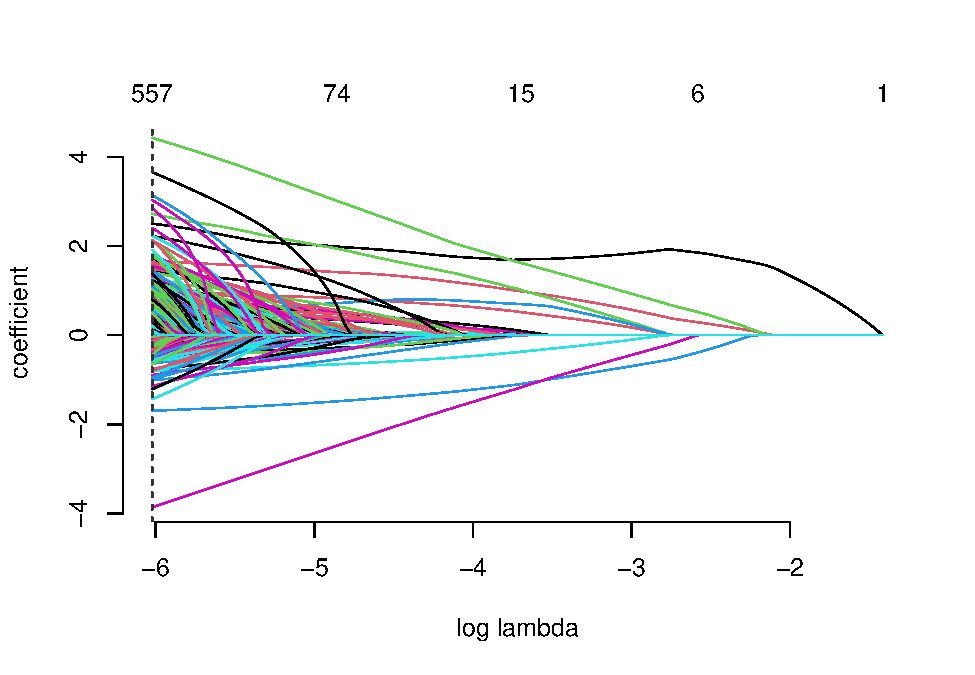
\includegraphics{final_bookdown_files/figure-latex/unnamed-chunk-23-1.pdf}

\hypertarget{hiper-parametro}{%
\subsection{Hiper parametro}\label{hiper-parametro}}

Automaticamente se elige el lambda que minimiza la devianza OOS.

\begin{Shaded}
\begin{Highlighting}[]
\CommentTok{\# Identificador para el lambda deseado}
\CommentTok{\# Valor del lambda deseado}
\CommentTok{\#lambda resultante}
\NormalTok{a\_lambda}\OtherTok{\textless{}{-}} \FunctionTok{colnames}\NormalTok{(}\FunctionTok{coef}\NormalTok{(cvlasso\_a, }\AttributeTok{select=}\StringTok{"min"}\NormalTok{))}
\NormalTok{cvlasso\_a}\SpecialCharTok{$}\NormalTok{gamlr}\SpecialCharTok{$}\NormalTok{lambda[a\_lambda]}
\end{Highlighting}
\end{Shaded}

\begin{verbatim}
##      seg100 
## 0.002426488
\end{verbatim}

\hypertarget{variables}{%
\subsection{Variables}\label{variables}}

A continuacion una tabla con los coeficientes que se selecciona para el CV LASSO. Que sorprendentemente solo fueron 561.

\begin{Shaded}
\begin{Highlighting}[]
\NormalTok{coefs}\OtherTok{\textless{}{-}}\FunctionTok{coef}\NormalTok{(cvlasso\_a, }\AttributeTok{select=}\StringTok{"min"}\NormalTok{, }\AttributeTok{k=}\DecValTok{2}\NormalTok{, }\AttributeTok{corrected=}\ConstantTok{TRUE}\NormalTok{)}
\NormalTok{coefs}\OtherTok{\textless{}{-}}\FunctionTok{as.data.frame}\NormalTok{(coefs[,}\DecValTok{1}\NormalTok{])}
\FunctionTok{names}\NormalTok{(coefs)}\OtherTok{\textless{}{-}}\StringTok{"valor"}
\NormalTok{coefs}\OtherTok{\textless{}{-}}\NormalTok{coefs }\SpecialCharTok{\%\textgreater{}\%} \FunctionTok{filter}\NormalTok{(valor }\SpecialCharTok{!=}\DecValTok{0}\NormalTok{)}
\NormalTok{modelvariables}\OtherTok{\textless{}{-}}\FunctionTok{row.names}\NormalTok{(coefs)}
\NormalTok{modelvariables}
\end{Highlighting}
\end{Shaded}

\begin{verbatim}
##   [1] "intercept"                      "lead_time"                     
##   [3] "arrival_date_year2015"          "arrival_date_year2017"         
##   [5] "arrival_date_monthDecember"     "arrival_date_monthJune"        
##   [7] "arrival_date_monthMarch"        "arrival_date_week_number43"    
##   [9] "arrival_date_day_of_month22"    "arrival_date_day_of_month30"   
##  [11] "stays_in_weekend_nights"        "stays_in_week_nights"          
##  [13] "adults"                         "mealHB"                        
##  [15] "mealUndefined"                  "countryAGO"                    
##  [17] "countryARE"                     "countryAUT"                    
##  [19] "countryBEL"                     "countryBGD"                    
##  [21] "countryBRA"                     "countryCHE"                    
##  [23] "countryCHN"                     "countryCPV"                    
##  [25] "countryDEU"                     "countryESP"                    
##  [27] "countryFIN"                     "countryFRA"                    
##  [29] "countryGBR"                     "countryGEO"                    
##  [31] "countryGGY"                     "countryGLP"                    
##  [33] "countryHKG"                     "countryHND"                    
##  [35] "countryIDN"                     "countryIRL"                    
##  [37] "countryISR"                     "countryITA"                    
##  [39] "countryJEY"                     "countryJPN"                    
##  [41] "countryKOR"                     "countryLTU"                    
##  [43] "countryLUX"                     "countryMAC"                    
##  [45] "countryMAR"                     "countryMDV"                    
##  [47] "countryMEX"                     "countryNGA"                    
##  [49] "countryNLD"                     "countryPAK"                    
##  [51] "countryPAN"                     "countryPOL"                    
##  [53] "countryPRT"                     "countryQAT"                    
##  [55] "countryRUS"                     "countrySAU"                    
##  [57] "countrySRB"                     "countrySWE"                    
##  [59] "countryTJK"                     "countryTUR"                    
##  [61] "countryZAF"                     "distribution_channel5"         
##  [63] "is_repeated_guest"              "previous_bookings_not_canceled"
##  [65] "reserved_room_typeE"            "reserved_room_typeP"           
##  [67] "assigned_room_typeB"            "assigned_room_typeI"           
##  [69] "assigned_room_typeP"            "booking_changes"               
##  [71] "deposit_typeB"                  "agent107"                      
##  [73] "agent11"                        "agent110"                      
##  [75] "agent118"                       "agent13"                       
##  [77] "agent132"                       "agent134"                      
##  [79] "agent14"                        "agent152"                      
##  [81] "agent155"                       "agent157"                      
##  [83] "agent16"                        "agent168"                      
##  [85] "agent17"                        "agent179"                      
##  [87] "agent191"                       "agent201"                      
##  [89] "agent214"                       "agent215"                      
##  [91] "agent22"                        "agent220"                      
##  [93] "agent23"                        "agent234"                      
##  [95] "agent240"                       "agent241"                      
##  [97] "agent242"                       "agent243"                      
##  [99] "agent248"                       "agent26"                       
## [101] "agent262"                       "agent27"                       
## [103] "agent281"                       "agent288"                      
## [105] "agent291"                       "agent307"                      
## [107] "agent308"                       "agent314"                      
## [109] "agent315"                       "agent32"                       
## [111] "agent332"                       "agent368"                      
## [113] "agent38"                        "agent390"                      
## [115] "agent40"                        "agent410"                      
## [117] "agent440"                       "agent56"                       
## [119] "agent6"                         "agent63"                       
## [121] "agent69"                        "agent7"                        
## [123] "agent8"                         "agent89"                       
## [125] "agent9"                         "agent94"                       
## [127] "company102"                     "company110"                    
## [129] "company112"                     "company153"                    
## [131] "company154"                     "company242"                    
## [133] "company275"                     "company280"                    
## [135] "company309"                     "company31"                     
## [137] "company321"                     "company350"                    
## [139] "company38"                      "company39"                     
## [141] "company392"                     "company40"                     
## [143] "company416"                     "company461"                    
## [145] "company478"                     "company486"                    
## [147] "company504"                     "company51"                     
## [149] "company513"                     "company68"                     
## [151] "company72"                      "company77"                     
## [153] "company88"                      "company94"                     
## [155] "companyNULL"                    "customer_typeTransient"        
## [157] "adr"                            "required_car_parking_spaces"   
## [159] "total_of_special_requests"      "dia_semviernes"                
## [161] "pascua_m2"                      "agent_company107_NULL"         
## [163] "agent_company110_NULL"          "agent_company118_NULL"         
## [165] "agent_company13_NULL"           "agent_company134_NULL"         
## [167] "agent_company155_NULL"          "agent_company17_NULL"          
## [169] "agent_company179_NULL"          "agent_company191_NULL"         
## [171] "agent_company214_NULL"          "agent_company234_NULL"         
## [173] "agent_company240_NULL"          "agent_company242_NULL"         
## [175] "agent_company248_NULL"          "agent_company250_NULL"         
## [177] "agent_company262_NULL"          "agent_company281_NULL"         
## [179] "agent_company291_NULL"          "agent_company307_NULL"         
## [181] "agent_company315_NULL"          "agent_company332_NULL"         
## [183] "agent_company368_NULL"          "agent_company38_NULL"          
## [185] "agent_company390_NULL"          "agent_company410_NULL"         
## [187] "agent_company440_NULL"          "agent_company56_NULL"          
## [189] "agent_company8_NULL"            "agent_company9_NULL"           
## [191] "agent_company94_NULL"           "agent_companyNULL_102"         
## [193] "agent_companyNULL_110"          "agent_companyNULL_112"         
## [195] "agent_companyNULL_153"          "agent_companyNULL_275"         
## [197] "agent_companyNULL_280"          "agent_companyNULL_281"         
## [199] "agent_companyNULL_309"          "agent_companyNULL_31"          
## [201] "agent_companyNULL_321"          "agent_companyNULL_350"         
## [203] "agent_companyNULL_38"           "agent_companyNULL_392"         
## [205] "agent_companyNULL_416"          "agent_companyNULL_461"         
## [207] "agent_companyNULL_478"          "agent_companyNULL_486"         
## [209] "agent_companyNULL_513"          "agent_companyNULL_68"          
## [211] "agent_companyNULL_77"           "agent_companyNULL_88"          
## [213] "agent_companyNULL_94"           "singles_adults"                
## [215] "dif_room"                       "weekmonthJune_27"              
## [217] "weekmonthOctober_43"            "weekmonthSeptember_40"         
## [219] "daymontApril_30"                "daymontApril_4"                
## [221] "daymontApril_5"                 "daymontApril_6"                
## [223] "daymontAugust_17"               "daymontAugust_27"              
## [225] "daymontDecember_16"             "daymontDecember_18"            
## [227] "daymontDecember_6"              "daymontFebruary_1"             
## [229] "daymontFebruary_27"             "daymontFebruary_8"             
## [231] "daymontJanuary_10"              "daymontJuly_1"                 
## [233] "daymontJuly_10"                 "daymontJuly_16"                
## [235] "daymontJuly_17"                 "daymontJuly_2"                 
## [237] "daymontJuly_22"                 "daymontJuly_23"                
## [239] "daymontJuly_28"                 "daymontJuly_5"                 
## [241] "daymontJuly_7"                  "daymontJune_10"                
## [243] "daymontJune_21"                 "daymontJune_26"                
## [245] "daymontJune_8"                  "daymontMarch_29"               
## [247] "daymontMay_15"                  "daymontMay_26"                 
## [249] "daymontMay_27"                  "daymontNovember_11"            
## [251] "daymontNovember_12"             "daymontNovember_23"            
## [253] "daymontOctober_12"              "daymontOctober_13"             
## [255] "daymontOctober_14"              "daymontOctober_22"             
## [257] "daymontOctober_25"              "daymontOctober_26"             
## [259] "daymontOctober_27"              "daymontOctober_8"              
## [261] "daymontSeptember_10"            "daymontSeptember_25"           
## [263] "weekdaymonthApril_15_4"         "weekdaymonthApril_15_5"        
## [265] "weekdaymonthApril_15_6"         "weekdaymonthAugust_33_14"      
## [267] "weekdaymonthAugust_34_17"       "weekdaymonthAugust_35_27"      
## [269] "weekdaymonthAugust_35_29"       "weekdaymonthDecember_49_5"     
## [271] "weekdaymonthDecember_50_6"      "weekdaymonthDecember_51_16"    
## [273] "weekdaymonthDecember_53_26"     "weekdaymonthFebruary_10_28"    
## [275] "weekdaymonthFebruary_8_24"      "weekdaymonthFebruary_9_27"     
## [277] "weekdaymonthFebruary_9_28"      "weekdaymonthJanuary_1_3"       
## [279] "weekdaymonthJanuary_1_4"        "weekdaymonthJanuary_1_6"       
## [281] "weekdaymonthJuly_27_1"          "weekdaymonthJuly_27_2"         
## [283] "weekdaymonthJuly_27_3"          "weekdaymonthJuly_28_5"         
## [285] "weekdaymonthJuly_28_7"          "weekdaymonthJuly_29_16"        
## [287] "weekdaymonthJuly_29_17"         "weekdaymonthJuly_30_22"        
## [289] "weekdaymonthJuly_30_23"         "weekdaymonthJuly_31_28"        
## [291] "weekdaymonthJune_24_10"         "weekdaymonthJune_24_8"         
## [293] "weekdaymonthJune_26_21"         "weekdaymonthJune_27_26"        
## [295] "weekdaymonthMarch_11_14"        "weekdaymonthMarch_13_25"       
## [297] "weekdaymonthMarch_9_1"          "weekdaymonthMay_21_15"         
## [299] "weekdaymonthMay_22_26"          "weekdaymonthMay_22_27"         
## [301] "weekdaymonthNovember_46_11"     "weekdaymonthNovember_46_12"    
## [303] "weekdaymonthNovember_48_20"     "weekdaymonthNovember_48_23"    
## [305] "weekdaymonthNovember_48_27"     "weekdaymonthNovember_49_27"    
## [307] "weekdaymonthOctober_40_2"       "weekdaymonthOctober_41_8"      
## [309] "weekdaymonthOctober_42_12"      "weekdaymonthOctober_42_13"     
## [311] "weekdaymonthOctober_42_14"      "weekdaymonthOctober_42_17"     
## [313] "weekdaymonthOctober_42_9"       "weekdaymonthOctober_43_17"     
## [315] "weekdaymonthOctober_43_22"      "weekdaymonthOctober_43_23"     
## [317] "weekdaymonthOctober_44_25"      "weekdaymonthOctober_44_26"     
## [319] "weekdaymonthOctober_44_27"      "weekdaymonthSeptember_36_5"    
## [321] "weekdaymonthSeptember_37_10"    "weekdaymonthSeptember_37_4"    
## [323] "month_diasemApril_lunes"        "month_diasemAugust_domingo"    
## [325] "month_diasemAugust_sabado"      "month_diasemDecember_viernes"  
## [327] "month_diasemJuly_miercoles"     "month_diasemJune_martes"       
## [329] "month_diasemMarch_domingo"      "month_diasemMay_jueves"        
## [331] "month_diasemOctober_sabado"     "week_diasem1_sabado"           
## [333] "week_diasem12_domingo"          "week_diasem12_lunes"           
## [335] "week_diasem15_lunes"            "week_diasem15_martes"          
## [337] "week_diasem15_miercoles"        "week_diasem24_viernes"         
## [339] "week_diasem27_domingo"          "week_diasem27_miercoles"       
## [341] "week_diasem28_sabado"           "week_diasem29_sabado"          
## [343] "week_diasem30_jueves"           "week_diasem31_lunes"           
## [345] "week_diasem33_sabado"           "week_diasem37_jueves"          
## [347] "week_diasem37_martes"           "week_diasem38_martes"          
## [349] "week_diasem39_sabado"           "week_diasem40_lunes"           
## [351] "week_diasem40_sabado"           "week_diasem41_martes"          
## [353] "week_diasem42_lunes"            "week_diasem44_domingo"         
## [355] "week_diasem45_sabado"           "week_diasem48_viernes"         
## [357] "week_diasem53_lunes"            "week_diasem7_sabado"           
## [359] "week_diasem8_martes"            "tasa_canc"                     
## [361] "market_dist3_TA_TO"             "market_distOfflineTA_TO_TA_TO" 
## [363] "cust_depostiTransient_B"        "cust_segmentContract_3"        
## [365] "cust_segmentContract_7"         "cust_segmentTransient_7"       
## [367] "cust_segmentTransient-Party_1"  "cust_segmentTransient-Party_3" 
## [369] "cust_segmentTransient-Party_7"  "lead_depositA_[ 16, 59)"       
## [371] "lead_depositA_[ 59,146)"        "lead_depositA_[146,737]"       
## [373] "lead_depositB_[ 59,146)"        "lead_week1_[ 59,146)"          
## [375] "lead_week10_[146,737]"          "lead_week12_[ 59,146)"         
## [377] "lead_week13_[  0, 16)"          "lead_week18_[  0, 16)"         
## [379] "lead_week18_[ 59,146)"          "lead_week2_[  0, 16)"          
## [381] "lead_week2_[ 59,146)"           "lead_week20_[ 59,146)"         
## [383] "lead_week22_[146,737]"          "lead_week23_[ 16, 59)"         
## [385] "lead_week24_[ 16, 59)"          "lead_week3_[  0, 16)"          
## [387] "lead_week3_[ 59,146)"           "lead_week3_[146,737]"          
## [389] "lead_week31_[ 16, 59)"          "lead_week32_[  0, 16)"         
## [391] "lead_week32_[ 16, 59)"          "lead_week32_[ 59,146)"         
## [393] "lead_week35_[ 16, 59)"          "lead_week4_[146,737]"          
## [395] "lead_week40_[ 59,146)"          "lead_week42_[  0, 16)"         
## [397] "lead_week42_[ 16, 59)"          "lead_week42_[ 59,146)"         
## [399] "lead_week43_[ 59,146)"          "lead_week44_[  0, 16)"         
## [401] "lead_week44_[ 59,146)"          "lead_week44_[146,737]"         
## [403] "lead_week45_[ 59,146)"          "lead_week48_[  0, 16)"         
## [405] "lead_week48_[ 59,146)"          "lead_week49_[ 16, 59)"         
## [407] "lead_week49_[ 59,146)"          "lead_week5_[  0, 16)"          
## [409] "lead_week5_[ 59,146)"           "lead_week50_[  0, 16)"         
## [411] "lead_week50_[ 59,146)"          "lead_week51_[146,737]"         
## [413] "lead_week52_[ 59,146)"          "lead_week52_[146,737]"         
## [415] "lead_week53_[146,737]"          "lead_week6_[  0, 16)"          
## [417] "lead_week6_[ 59,146)"           "lead_week6_[146,737]"          
## [419] "lead_week7_[ 59,146)"           "lead_week8_[  0, 16)"          
## [421] "lead_week8_[146,737]"           "lead_week9_[  0, 16)"          
## [423] "meal_reservBB_D"                "meal_reservFB_A"               
## [425] "meal_reservSC_A"                "meal_reservSC_D"               
## [427] "meal_reservSC_F"                "meal_reservSC_P"               
## [429] "meal_reservUndefined_D"         "country_monthAGO_April"        
## [431] "country_monthAGO_February"      "country_monthALB_April"        
## [433] "country_monthAND_January"       "country_monthAUS_April"        
## [435] "country_monthAUS_February"      "country_monthAUS_March"        
## [437] "country_monthAUT_February"      "country_monthAUT_July"         
## [439] "country_monthAUT_March"         "country_monthAUT_October"      
## [441] "country_monthAZE_March"         "country_monthBEL_August"       
## [443] "country_monthBGR_May"           "country_monthBLR_January"      
## [445] "country_monthBRA_April"         "country_monthCHE_April"        
## [447] "country_monthCHE_July"          "country_monthCHL_April"        
## [449] "country_monthCHL_December"      "country_monthCHN_December"     
## [451] "country_monthCHN_January"       "country_monthCHN_July"         
## [453] "country_monthCHN_May"           "country_monthCHN_October"      
## [455] "country_monthCOL_November"      "country_monthCOL_September"    
## [457] "country_monthCYP_August"        "country_monthCYP_May"          
## [459] "country_monthCZE_August"        "country_monthCZE_October"      
## [461] "country_monthDEU_April"         "country_monthDEU_December"     
## [463] "country_monthDEU_October"       "country_monthEGY_February"     
## [465] "country_monthESP_April"         "country_monthESP_December"     
## [467] "country_monthESP_June"          "country_monthFIN_May"          
## [469] "country_monthFRA_April"         "country_monthFRA_January"      
## [471] "country_monthFRA_June"          "country_monthFRA_March"        
## [473] "country_monthFRA_May"           "country_monthFRA_November"     
## [475] "country_monthGBR_August"        "country_monthGBR_June"         
## [477] "country_monthGBR_October"       "country_monthGGY_December"     
## [479] "country_monthGHA_November"      "country_monthGIB_August"       
## [481] "country_monthGIB_March"         "country_monthGLP_December"     
## [483] "country_monthGRC_April"         "country_monthGRC_March"        
## [485] "country_monthHND_February"      "country_monthHRV_January"      
## [487] "country_monthHRV_March"         "country_monthHUN_August"       
## [489] "country_monthHUN_January"       "country_monthHUN_November"     
## [491] "country_monthIDN_December"      "country_monthIND_June"         
## [493] "country_monthIRL_July"          "country_monthIRL_June"         
## [495] "country_monthIRL_May"           "country_monthIRL_October"      
## [497] "country_monthIRN_February"      "country_monthIRN_March"        
## [499] "country_monthITA_December"      "country_monthITA_July"         
## [501] "country_monthITA_September"     "country_monthJEY_September"    
## [503] "country_monthJPN_December"      "country_monthKAZ_January"      
## [505] "country_monthKEN_March"         "country_monthKOR_August"       
## [507] "country_monthKOR_February"      "country_monthKOR_May"          
## [509] "country_monthLUX_December"      "country_monthLUX_February"     
## [511] "country_monthLUX_November"      "country_monthMAR_August"       
## [513] "country_monthMAR_February"      "country_monthMDV_November"     
## [515] "country_monthMEX_July"          "country_monthMKD_October"      
## [517] "country_monthMOZ_June"          "country_monthNGA_March"        
## [519] "country_monthNLD_February"      "country_monthNLD_November"     
## [521] "country_monthNOR_July"          "country_monthNOR_October"      
## [523] "country_monthOMN_January"       "country_monthPER_March"        
## [525] "country_monthPER_November"      "country_monthPOL_March"        
## [527] "country_monthPRI_December"      "country_monthPRT_August"       
## [529] "country_monthPRT_January"       "country_monthPRT_May"          
## [531] "country_monthPRT_November"      "country_monthPRT_October"      
## [533] "country_monthPRT_September"     "country_monthQAT_April"        
## [535] "country_monthROU_February"      "country_monthROU_October"      
## [537] "country_monthRUS_April"         "country_monthRUS_March"        
## [539] "country_monthSAU_February"      "country_monthSGP_January"      
## [541] "country_monthSVN_March"         "country_monthSWE_December"     
## [543] "country_monthSWE_February"      "country_monthSWE_March"        
## [545] "country_monthTHA_February"      "country_monthTHA_June"         
## [547] "country_monthTJK_May"           "country_monthTUN_March"        
## [549] "country_monthTUN_October"       "country_monthTUR_July"         
## [551] "country_monthTWN_February"      "country_monthTZA_September"    
## [553] "country_monthURY_March"         "country_monthVEN_January"      
## [555] "country_monthVEN_September"     "country_monthZAF_October"      
## [557] "country_monthZMB_April"
\end{verbatim}

\hypertarget{log-loss-test-oos}{%
\subsection{LOG LOSS test OOS}\label{log-loss-test-oos}}

Ahora pruebo el error log loss del lasso

\begin{Shaded}
\begin{Highlighting}[]
\CommentTok{\#Predicciones}
\NormalTok{lasso\_score }\OtherTok{\textless{}{-}} \FunctionTok{predict}\NormalTok{(cvlasso\_a,}
               \AttributeTok{newdata =}\NormalTok{ Xb,}
               \AttributeTok{type=}\StringTok{"response"}\NormalTok{,}
               \AttributeTok{select =} \StringTok{"min"}\NormalTok{ )}


\CommentTok{\#dataframe}
\NormalTok{lasso\_validation }\OtherTok{\textless{}{-}} \FunctionTok{data.frame}\NormalTok{(y, lasso\_score)}
\FunctionTok{colnames}\NormalTok{(lasso\_validation)[}\DecValTok{2}\NormalTok{] }\OtherTok{\textless{}{-}} \FunctionTok{c}\NormalTok{(}\StringTok{\textquotesingle{}lasso\_score\textquotesingle{}}\NormalTok{)}

\FunctionTok{library}\NormalTok{(MLmetrics)}
\end{Highlighting}
\end{Shaded}

\begin{verbatim}
## 
## Attaching package: 'MLmetrics'
\end{verbatim}

\begin{verbatim}
## The following object is masked from 'package:base':
## 
##     Recall
\end{verbatim}

\begin{Shaded}
\begin{Highlighting}[]
\FunctionTok{LogLoss}\NormalTok{(lasso\_validation}\SpecialCharTok{$}\NormalTok{lasso\_score,lasso\_validation}\SpecialCharTok{$}\NormalTok{y)}
\end{Highlighting}
\end{Shaded}

\begin{verbatim}
## [1] 0.3074453
\end{verbatim}

Nos dio un error sorprendetemente muy pequeño. Con este modelo logramos realizar un error de 0.41872 y 0.42131 en los datos de test de Kaggle.

\hypertarget{xgboosting}{%
\section{XGBOOSTING}\label{xgboosting}}

Sin embargo, para ganar el concurso optamos por explorar otros modelos que generalmente tienen mayor potencial de ganar este tipo de concursos: XG boosting.

En este caso, se eligieron los hiperparametros mediante un tuning manual explorando el comportamiento del error cuando se fijaban todos los hp excepto uno. De esta manera se fijo la profunidad máxima del arbol en 6 y el learning rate en .06.

Debido a la alta cantidad de variables de las bases de datos (y pues que muchas son poco informativas) el colsample por cada arbol generado es alto: del 70\%. De haber tenido solo variables muy informativas pues bajariamos ese porcentaje, sin embargo quicimos explitar la capacidad del modelo de seleccionar por si solo las variables.

\begin{Shaded}
\begin{Highlighting}[]
\CommentTok{\# Preparar la base de entrenamiento}
\FunctionTok{library}\NormalTok{(xgboost)}
\end{Highlighting}
\end{Shaded}

\begin{verbatim}
## 
## Attaching package: 'xgboost'
\end{verbatim}

\begin{verbatim}
## The following object is masked from 'package:plotly':
## 
##     slice
\end{verbatim}

\begin{verbatim}
## The following object is masked from 'package:dplyr':
## 
##     slice
\end{verbatim}

\begin{Shaded}
\begin{Highlighting}[]
\NormalTok{dtrain }\OtherTok{\textless{}{-}} \FunctionTok{xgb.DMatrix}\NormalTok{(Xa, }\AttributeTok{label =}\NormalTok{ Ya) }
\CommentTok{\# Label es el target}
\CommentTok{\# Preparar la base de validación}

\NormalTok{dtest }\OtherTok{\textless{}{-}} \FunctionTok{xgb.DMatrix}\NormalTok{(Xb, }\AttributeTok{label =}\NormalTok{ y)}
\NormalTok{watchlist }\OtherTok{\textless{}{-}} \FunctionTok{list}\NormalTok{(}\AttributeTok{train =}\NormalTok{ dtrain, }\AttributeTok{eval =}\NormalTok{ dtest) }
\CommentTok{\# Para evaluar el performance del modelo}


\CommentTok{\# Entrenamiento del modelo}

\NormalTok{param }\OtherTok{\textless{}{-}} \FunctionTok{list}\NormalTok{(}\AttributeTok{max\_depth =} \DecValTok{6}\NormalTok{, }\AttributeTok{learning\_rate =} \FloatTok{0.06}\NormalTok{, }
              \AttributeTok{objective =} \StringTok{"binary:logistic"}\NormalTok{,}
              \AttributeTok{eval\_metric =} \StringTok{"logloss"}\NormalTok{, }\AttributeTok{subsample =} \FloatTok{0.6}\NormalTok{, }\AttributeTok{colsample\_bytree =} \FloatTok{0.7}\NormalTok{)}


\NormalTok{xgb\_model }\OtherTok{\textless{}{-}} \FunctionTok{xgb.train}\NormalTok{(}\AttributeTok{params =}\NormalTok{ param, dtrain, }
                       \AttributeTok{early\_stopping\_rounds =}  \DecValTok{10}\NormalTok{, }
                       \AttributeTok{nrounds =} \DecValTok{300}\NormalTok{,}
\NormalTok{                 watchlist)}
\CommentTok{\# Predicción}
\NormalTok{xgb\_pred }\OtherTok{\textless{}{-}} \FunctionTok{predict}\NormalTok{(xgb\_model, Xb)}
\NormalTok{XGpred}\OtherTok{\textless{}{-}}\FunctionTok{data.frame}\NormalTok{(y, xgb\_pred)}
\FunctionTok{colnames}\NormalTok{(XGpred)}\OtherTok{\textless{}{-}}\FunctionTok{c}\NormalTok{(}\StringTok{"y"}\NormalTok{,}\StringTok{"xgb\_pred"}\NormalTok{)}
\end{Highlighting}
\end{Shaded}

Se muestran las evaluaciones del modelo, tanto in sample como out of sample, para las primeras y últimas iteraciones.

\begin{Shaded}
\begin{Highlighting}[]
\FunctionTok{LogLoss}\NormalTok{(XGpred}\SpecialCharTok{$}\NormalTok{xgb\_pred,XGpred}\SpecialCharTok{$}\NormalTok{y)}
\end{Highlighting}
\end{Shaded}

\begin{verbatim}
## [1] 0.246542
\end{verbatim}

Este modelo logró ganar el concurso con un error en los datasets de kaggle de 0.37598 y 0.37401.

\hypertarget{conclusiones}{%
\chapter{Conclusiones}\label{conclusiones}}

\begin{itemize}
\item
  Los modelos lineales nos sirvieron para ir explorando la utilidad de las variables, parámetros y las caracteristicas del modelo sin embargo, una vez descubierto los insights pues podemos optar por modelos más competitivos.
\item
  Como vimos en clase el EDA se debe hacer después de un CV para evitar encontrar hallazgos que generalizen poco.
\item
  El usar matrices ralas nos permitio experimentar muy rapido con los modelos pues reducen el tiempo de entrenamiento. Sin embargo debemos tratar las bases de datos con mucho cuidado. Por ejemplo, se necesitavan nivelar las columnas para que las matrices tuvieran las mismas dimensiones.
\item
  Se puede explotar al máximo la capacidad de cada modelo de ML de seleccionar las variables (y en consecuencia de crear bases de datos de alta dimensión) sin embargo se debe comprender el cómo lo hacen. En nuestro caso, esto implicaba indicarle al modelo que queremos un colsample por cada arbol alto: del 70\% y que debemos limitar el tamaño de cada arbol en no más de 6 niveles.
\end{itemize}

  \bibliography{book.bib,packages.bib}

\end{document}
